%!TEX root = main.tex

\section{\vr video-specific QoE model}
\label{sec:jnd}

We first present a QoE model that estimates the subjective user experience when watching a \vr video.
We build the model on an existing QoE model for non-\vr video streaming, and incorporate the new \vr video-specific factors (\S\ref{subsec:opportunities}).
We begin with a brief introduction of the traditional video QoE model (\S\ref{subsec:jnd:pspnr}), then explain the general approach to incorporate the new factors (\S\ref{subsec:jnd:framework}), and finally provide details of how the new \vr video-specific factors affect the perceived QoE (\S\ref{subsec:jnd:details}).

\subsection{PSPNR and JND}
\label{subsec:jnd:pspnr}

\jc{need to tighten the text}

Peak Signal-to-Perceptible-Noise Ratio (PSPNR) \cite{PSPNR} is an widely-accepted metric to measure perceived quality. It is defined based on Just-Noticeable-Distortion (JND) theory \cite{JND}. Given the original video frame and a compressed video frame, user can notice their difference only if the difference between them is above a visibility threshold. When the different is under this threshold, it will not detected by user. This threshold is called Just-Noticeable-Distortion.

Based on JND theory, PSPNR is defined by accumulating error of each pixel which can be detected by user:

\begin{alignat}{2}\
\label{f1} PSPNR = 20 \times \log_{10}\frac{255}{\sqrt{PMSE}}
\end{alignat}
\begin{alignat}{2}\
PMSE=E\{ \left[ |p(x, y) - \hat{p}(x, y)| - JND(x, y)\right]^2 \times \Delta (x, y)\}
\end{alignat}
\begin{alignat}{2}\
\Delta (x, y) =\left\{
\begin{aligned}
1, & &|p(x, y) - \hat{p}(x, y)| > JND(x, y) \\
0, & &|p(x, y) - \hat{p}(x, y)| \le JND(x, y)
\end{aligned}
\right.
\end{alignat}

where $p(x, y)$ and $\hat{p}(x, y)$ are value of pixel $(x, y)$ in original video frame and compressed video frame. $JND(x, y)$ is the visibility threshold of pixel $(x, y)$.

Compared with PSNR (which is widely used in evaluating video / image quality), the core difference of PSPNR is introducing a term $JND(x, y)$ for each pixel $(x, y)$. So how to compute JND for each pixel $(x, y)$ is an important issue. We will present our JND computation in the following section.

The just-noticeable distortion (JND) provides cues for measuring the visibility of the Human Vision System (HVS). JND refers to the maximum distortion which cannot be perceived by human. It describes the perceptual redundancy of the picture by providing the visibility threshold. The JND model generally exploits the visibility of the minimally perceptible distortion.

JND has been well-studied in traditional video display since 1995. The most basic and solid research is about the relationship between content luminance and JND. \cite{luminance1}  and \cite{PSPNR} prove that content with moderate content luminance have low JND value, while content with very high or very low content luminance have high JND value. 


In recent years, based on the insight of content luminance - JND relationship, researchers have explored some more factors which are also related to JND, such as texture complexity, viewpoint-object distance (\cite{PSPNR}, \cite{distance}) and some other factors. Although the relationship between multiple JND factors may be complex, for simplicity, we can decouple them into several single factors. For example, \cite{distance} set up a user study to test the JND value with the combined effect of content luminance and viewpoint-object distance. The result proves that viewpoint-object distance can be considered independently from content luminance. It can be regarded as a coefficient which can be directly multiplied on JND value computed by content luminance. Based on this insight, JND computation for multiple factors is decoupled into several single factors. This significantly simplify the JND computation.

\subsection{JND for \vr videos}
\label{subsec:jnd:framework}


In VR display, user experience is very different because 3 new factors should be taken into consideration: (1) viewpoint moving decreases visual acuity, (2) low Depth-of-Field decreases visual acuity and (3) light / dark adaptation decreases visual acuity. So previous JND model for traditional video display can not be directly applied on VR video display. Moreover, it is unknown that (1) how these new factors influence JND with combined effect of old factors, and (2) if they can also be decoupled into several single factors, like viewpoint-object distance \cite{distance}.

Strictly answering these 2 questions needs to test JND value for each possible combinations of all factors (including all possible luminance, texture, viewpoint-object distance, viewpoint moving speed, Depth-of-Field and light / dark adaptation, which make up a 6-dimension feature space), which is not practical for a real-world user study. For simplicity, we imitate the user study in \cite{distance}, which makes only 2 factors variable and other 4 factors fixed, then we can know how is the combined effect of the 2 factors to JND, and if they can be decoupled to 2 single factors which independently influence JND.

So we present 3 user studies: (1) JND v.s. luminance \& viewpoint moving speed. (2) JND v.s. luminance \& depth of field. (3) JND v.s. luminance \& light / dark adaptation. We evaluate the effect of 3 VR-only factors to JND, each with combined effect of luminance, since luminance is the most well-studied JND factor.

We conduct the user study using real Head Mounted Device (HMD). Parameters of proposed HMD are listed as Table \ref{table1}:

\begin{table}[h]
\centering
\caption{HMD Parameters}\label{table1}
\begin{tabular}{|p{3.5cm}|p{3.5cm}|}
\hline
Equipment & Oculus GO\\
CPU & Xiaolong 821 customized drive Edition\\
Memory & 3GB\\
Screen Resolution & 2560 $\times$ 1440\\
Refresh Rate & 72Hz\\
Fixed pupil distance & 63.5mm\\
\hline
\end{tabular}
\end{table}

X subjects participated in the experiments, including X males and X females. All of them were in their twenties. The subjects obtained extensive practice during the experiments.

In this paper, we imitate the human visibility experiments in \cite{PSPNR}. In the experiment, a small square area, 32 x 32 pixels, is located in the center of a flat field of constant grey level (luminance). For each possible grey level (luminance) of the square area, the noises of fixed amplitude are randomly added to or subtracted from the pixels within the square area. Through varying the amplitude of the noise, the visibility threshold for each grey level is determined when the square region contaminated by the noises is just noticeable. 


\subsection{Profiling \vrjnd}
\label{subsec:jnd:details}

\mypara{Methodology}
\jc{explain the methodology here:
\begin{itemize}
\item briefly explain the human-based experiment (irb-approved)
\item how single-factor impact is measured? what default values are used while changing on one dimension at a time?
\item how mutual independence was tested?
\end{itemize}}

\mypara{Impact of viewpoint moving speed}
\jc{briefly explain Figure~\ref{JNDspeed-track} and what the correlation looks like (non-linearity? non-monotonicity? any suprising trend?)}

\begin{figure}
  \centering
  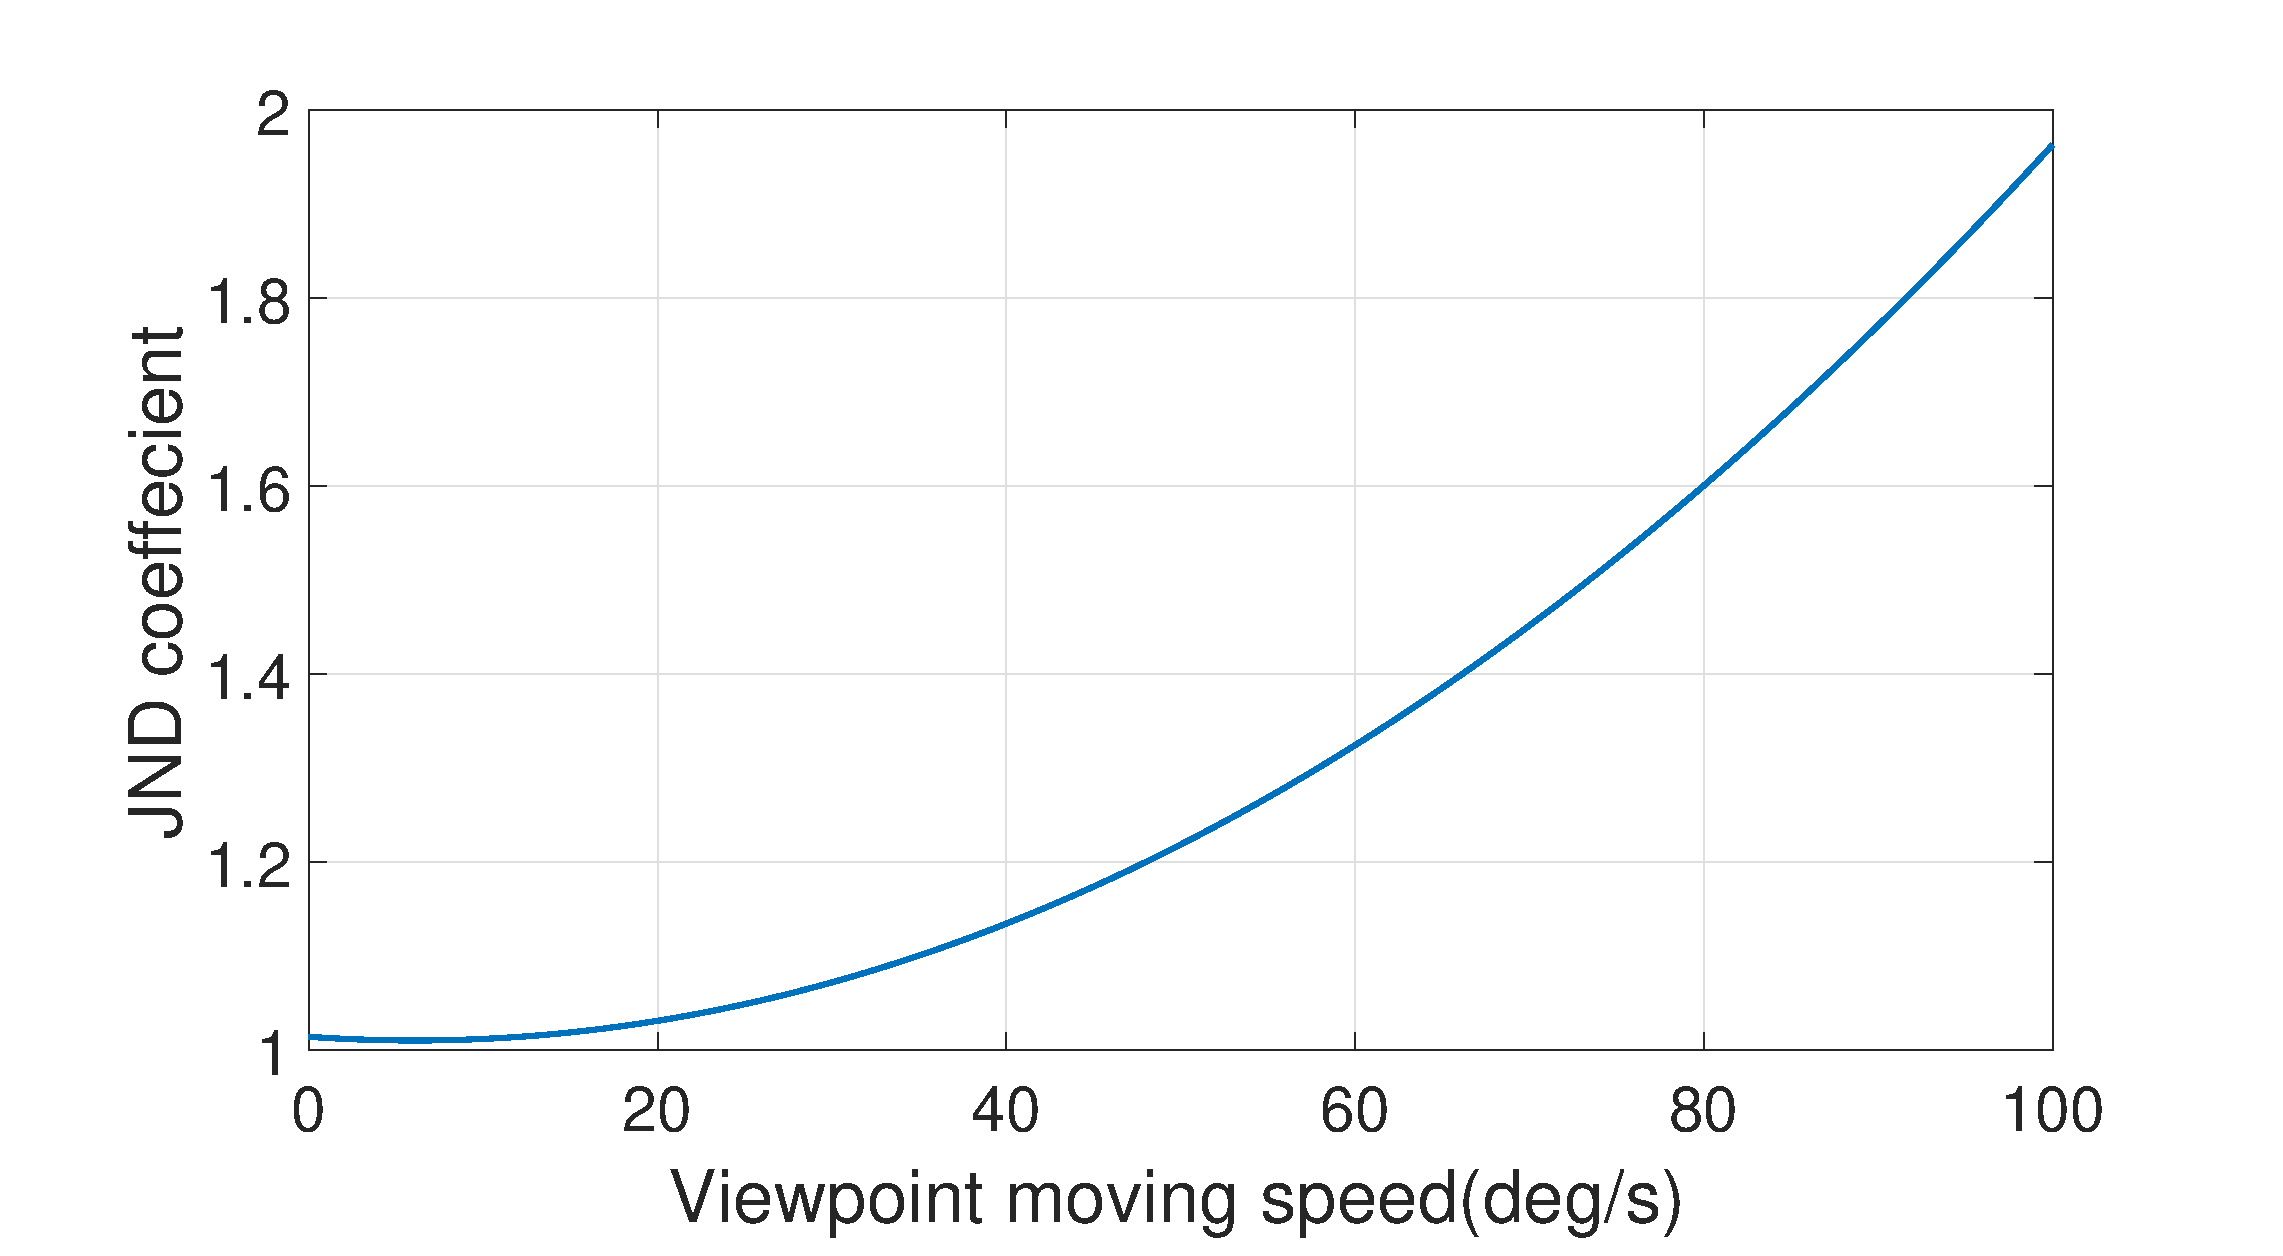
\includegraphics[width=2.5in]{images/JNDspeed.eps}
  \caption{$f_{track}(v)$, the JND coefficient of viewpoint moving speed.}
  \label{JNDspeed-track}
  \end{figure}

\mypara{Impact of switch of luminance}
\jc{show a similar graph of Figure~\ref{JNDspeed-track} to show the impact of changes of luminance and JND}

\mypara{Impact of changes of depth of field}
\jc{show a similar graph of Figure~\ref{JNDspeed-track} to show the impact of difference of DoF and JND}

\mypara{Mutual independence test}
\jc{show the 3D graphs and explain why the shapes confirm their impact on JDN is mutually independent.}






